\documentclass[letterpaper,12pt,conference]{ieeeconf}

\IEEEoverridecommandlockouts
\overrideIEEEmargins

\usepackage{graphicx}
\usepackage{amsmath,amssymb}
\usepackage{bm}
\usepackage{booktabs}
\usepackage[hyphens]{url}
\usepackage{hyperref}
\hypersetup{
  colorlinks=true,
  urlcolor=magenta,
  linkcolor=black,
  citecolor=black
}

\usepackage{textcomp}
\usepackage{xcolor} 

\title{\LARGE \bf
Adaptive Traffic Signal Control Using
Demand Forecasting and Rolling-Horizon Optimization
}

\author{
Younggun Kim$^{1}$ and Manuel A. Martinez Garcia$^{1}$%
\thanks{$^{1}$Department of Civil and Environmental Engineering,
University of California, Los Angeles (UCLA),
Los Angeles, California, USA.}%
}

\begin{document}

\maketitle
\thispagestyle{empty}
\pagestyle{empty}

%%%%%%%%%%%%%%%%%%%%%%%%%%%%%%%%%%%%%%%%%%%%%%%%%%%%%%%%%%%%



\begin{abstract}
Traffic signal control plays an important role in managing
congestion and reducing vehicle delays at urban intersections.
Fixed-time controllers rely on predetermined timing plans, and
queue-responsive controllers react to observed queues, but
neither uses recurring temporal patterns in future arrivals. This
project proposes a forecast-informed signal controller that
integrates Transformer-based demand forecasting with
rolling-horizon optimization. In our isolated-intersection
simulation, vehicles follow the Intelligent Driver Model (IDM), so
queue discharge, queue storage, and clearance needs result from
car-following behavior rather than being assumed. We will compare
the proposed controller with fixed-time and queue-responsive
control under balanced demand, a directional demand shift,
detector failure, and heavy demand. By examining the optimizer's
internal queue model, we argue that forecasts can influence
signal decisions only when a queue is expected to clear within the
planning horizon, so the benefit of forecasting should depend on
how congested the intersection is. All codes used in this project is available at \url{https://github.com/Kimyounggun99/CEE281-term-project.git}.
\end{abstract}

%%%%%%%%%%%%%%%%%%%%%%%%%%%%%%%%%%%%%%%%%%%%%%%%%%%%%%%%%%%%
\begin{figure}[t]
    \centering
    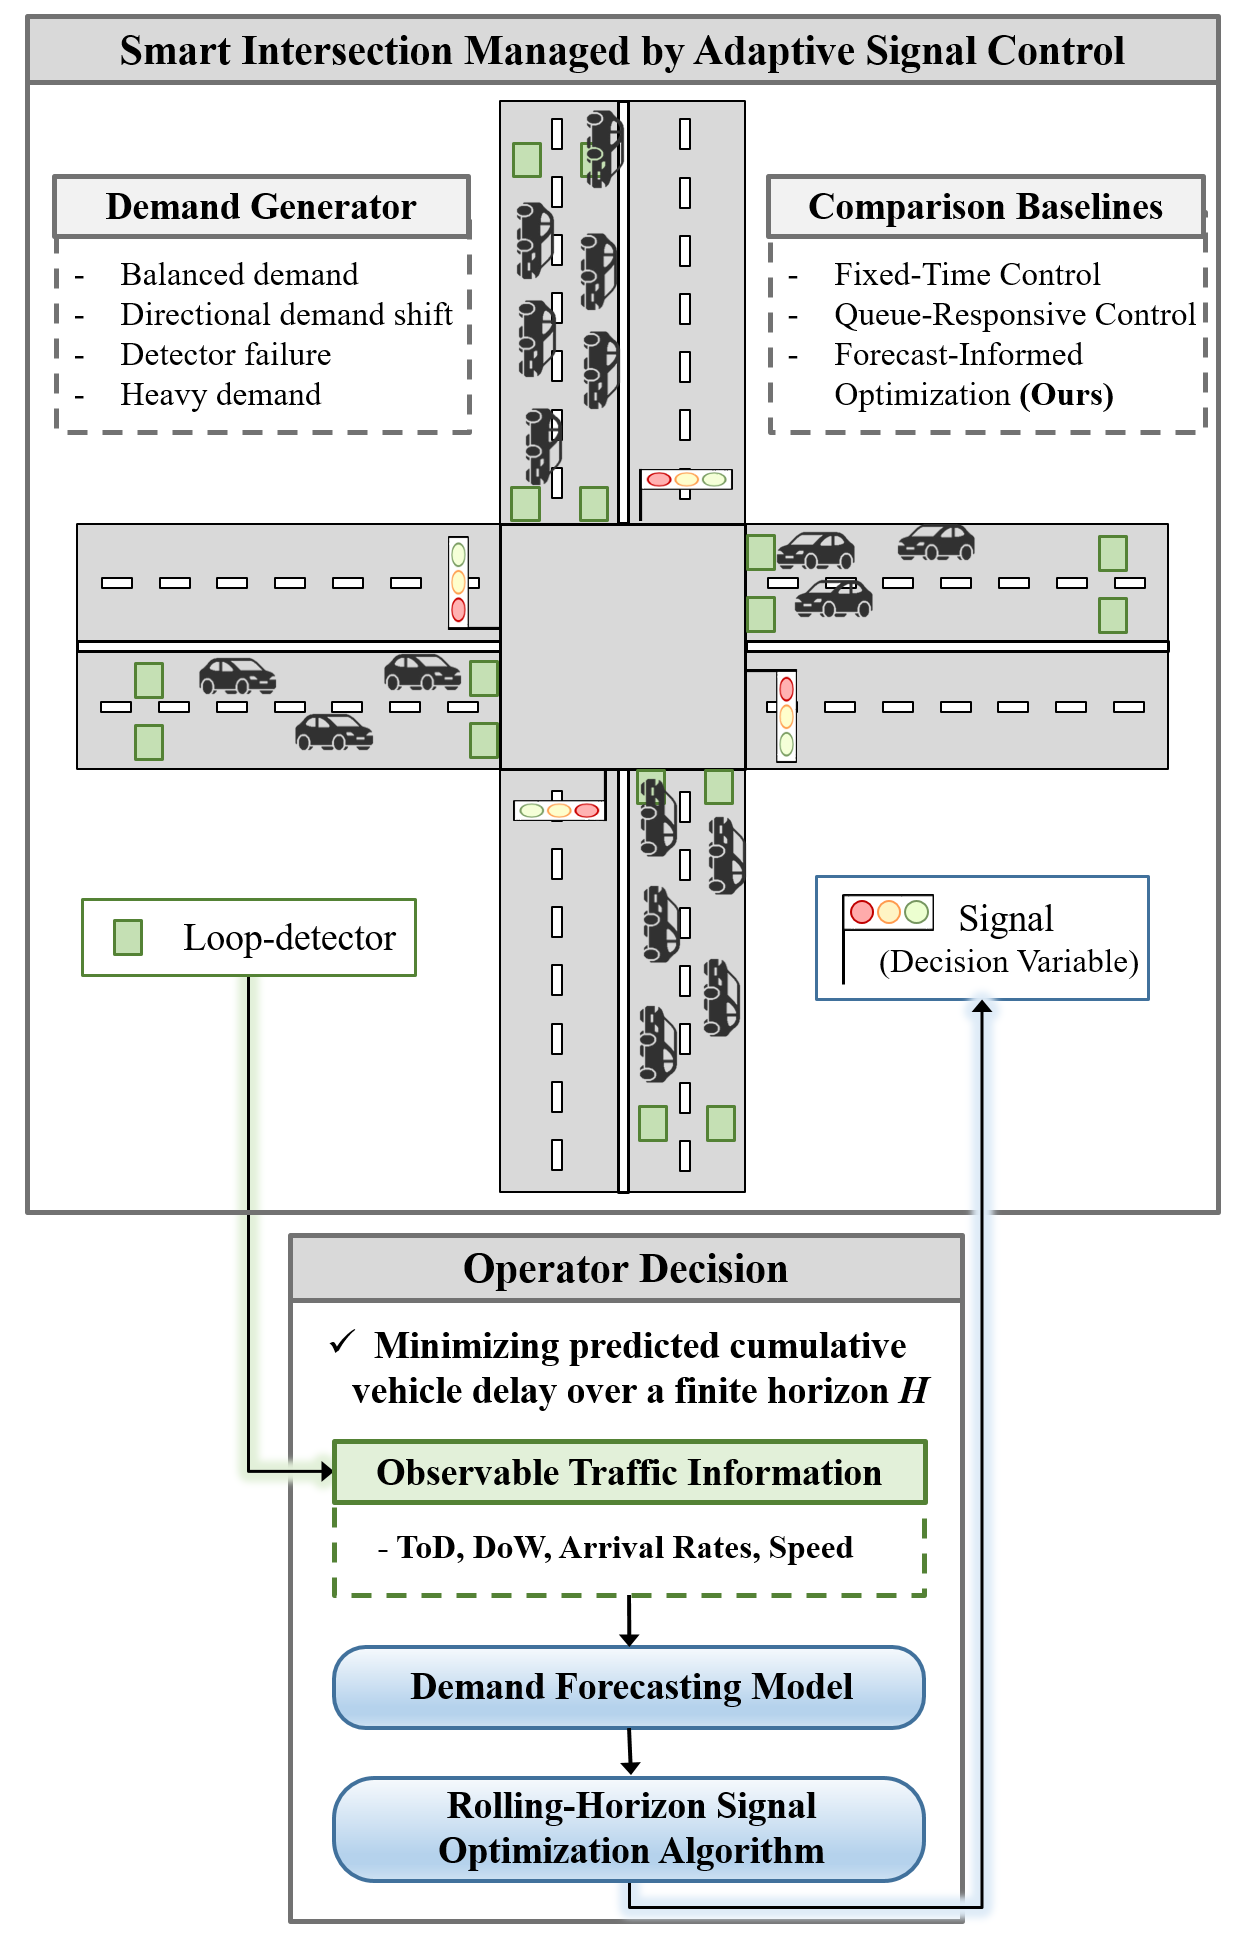
\includegraphics[width=0.9\linewidth]{System_Illustration.png}
    \caption{Overview of the proposed adaptive traffic signal control framework integrating Transformer-based demand forecasting and rolling-horizon optimization in an isolated intersection.}
    \label{fig:System_Illustration}
\end{figure}



\section{CORE CONCEPTS}
Our system environment and our approaches are summarized in Fig.~\ref{fig:System_Illustration}.
Our controller combines three ideas: how a signalized approach
serves vehicles, how individual vehicles move and form queues,
and how forecasts can be used inside an optimization. This section
explains each idea and its assumptions. Units are seconds (s),
meters (m), and vehicles (veh) unless stated otherwise.

\subsection{Flow, Headway, and Intersection Capacity}

Traffic flow $q$ [veh/s] is the number of vehicles passing a
point per unit time, and density $k$ [veh/m] is the number of
vehicles per unit length. They are linked by the mean speed
$\bar v$ [m/s] through $q=k\bar v$, and the average time headway
between vehicles is $1/q$ \cite{treiber2013}.

When a signal turns green, the vehicles in a queue cross the stop
line one after another. After the first few vehicles, which need
extra time to react and accelerate, the queue discharges with a
nearly constant headway $h_s$. The rate $S=1/h_s$ [veh/s/lane] is
the saturation flow. It is the key quantity in signal timing
because it tells us how many vehicles a given green time can
serve.

Let $\mathcal{A}$ denote the set of approaches. For approach
$i\in\mathcal{A}$ with $N_i$ lanes, arrival rate $\lambda_i$
[veh/s], and effective green time $g_i$ in a cycle of length $C$,
the capacity $c_i$, flow ratio $y_i$, and degree of saturation
$x_i$ are
\begin{equation}
c_i=\frac{N_i S\, g_i}{C},\qquad
y_i=\frac{\lambda_i}{N_i S},\qquad
x_i=\frac{\lambda_i}{c_i}.
\label{eq:capacity}
\end{equation}
The flow ratio is the fraction of the cycle that approach $i$
would need to be green. Each phase change also wastes time
(yellow, all-red, and start-up), which we call the lost time $L$
per cycle. All demand can therefore be served only if the sum of
critical flow ratios satisfies $Y=\sum_i y_i<1-L/C$.

Webster \cite{webster1958} derived the cycle length that
approximately minimizes delay, and the average delay caused by
waiting through red:
\begin{equation}
C_0=\frac{1.5L+5}{1-Y},\qquad
d_{u,i}=\frac{C(1-g_i/C)^2}{2(1-y_i)}.
\label{eq:webster}
\end{equation}
The author also showed that random arrivals add delay that grows without
bound as $x_i$ approaches one. Intuitively, when an approach has
spare capacity, a poor green allocation in one cycle is absorbed
in the next. Near capacity there is no spare green to recover, so
the same mistake leaves vehicles waiting for several cycles. This
is why information about future arrivals should matter most when
the intersection is busy but not yet overloaded.

\subsection{Queue Formation and Discharge}

Queues are conveniently described with cumulative counts. Let
$A_i(t)$ be the number of vehicles that have arrived at approach
$i$ by time $t$, and $D_i(t)$ the number that have departed. The
number waiting is $Q_i(t)=A_i(t)-D_i(t)$, and the area between the
two curves, $\int Q_i\,dt$ [veh$\cdot$s], equals total delay
\cite{newell1993}. During green, $D_i$ grows at most at rate
$N_iS$; during red it stays flat. If arrivals exceed capacity for
several cycles, the queue left after each green grows by
$\lambda_i-c_i$ per second, and re-timing alone cannot remove it.

Real queues also occupy space. Each stopped vehicle needs its
length $l$ plus a standstill gap $s_0$, so an approach of length
$\ell_a$ stores at most $\lfloor\ell_a/(l+s_0)\rfloor$ vehicles per
lane. During red, the back of the queue moves upstream as new
vehicles stop; after the light turns green, a start-up wave
travels backward through the queue as each driver begins to move.
Both boundaries move at the kinematic-wave speed
\cite{lighthill1955}
\begin{equation}
w=\frac{q_u-q_d}{k_u-k_d},
\label{eq:shock}
\end{equation}
where $(q_u,k_u)$ and $(q_d,k_d)$ are the traffic states on either
side of the boundary. When the queue tail reaches the upstream end
of the approach, arriving vehicles can no longer enter, and the
queue spills back beyond the modeled road. How quickly drivers
react and accelerate inside the queue, and therefore how fast it
discharges, depends on the car-following behavior described next
\cite{treiber2013}.

\subsection{Vehicle-Motion Model: the Intelligent Driver Model}

The IDM \cite{treiber2000} describes each driver as balancing two
goals: reaching a desired speed and keeping a safe gap behind the
vehicle ahead. We use it because its parameters have clear
physical meanings, it avoids collisions under normal settings,
and one equation reproduces free driving, following, stopping at
a red light, and accelerating away from a queue.

Vehicle $n$ has front-bumper position $x_n$ [m] and speed $v_n$
[m/s], with $\dot x_n=v_n$. The driver observes the net gap to the
leader $s_n=x_{n-1}-x_n-l$ [m] and the approach rate
$\Delta v_n=v_n-v_{n-1}$ [m/s], which is positive when closing in.
The acceleration is
\begin{equation}
\dot v_n=a\left[1-\left(\frac{v_n}{v_0}\right)^{\delta}
-\left(\frac{s^*(v_n,\Delta v_n)}{s_n}\right)^{2}\right],
\label{eq:idm}
\end{equation}
with the desired gap
\begin{equation}
s^*(v,\Delta v)=s_0+\max\!\left(0,\;vT+\frac{v\,\Delta v}{2\sqrt{ab}}\right).
\label{eq:sstar}
\end{equation}
Here $v_0$ is the desired speed [m/s], $T$ the desired time gap
[s], $s_0$ the standstill gap [m], $a$ the maximum acceleration
[m/s$^2$], $b$ the comfortable deceleration [m/s$^2$], and
$\delta$ [--] controls how acceleration fades near $v_0$.

The bracket in (\ref{eq:idm}) contains two competing effects. The
term $(v_n/v_0)^\delta$ lets the vehicle accelerate on an empty road
and stop accelerating near $v_0$. The term $(s^*/s_n)^2$ brakes the
vehicle when its gap is shorter than desired. The desired gap
grows with speed through $vT$, so faster drivers keep more
distance, and it grows with the closing speed $\Delta v$, so a
driver approaching a stopped vehicle brakes early and smoothly.
When the leader pulls away ($\Delta v<0$), the driver accelerates.

If all vehicles travel at the same constant speed,
$\dot v_n=\Delta v_n=0$, and (\ref{eq:idm}) gives the equilibrium
gap and flow
\begin{equation}
s_e(v)=\frac{s_0+vT}{\sqrt{1-(v/v_0)^{\delta}}},\qquad
Q_e(v)=\frac{v}{s_e(v)+l}.
\label{eq:equil}
\end{equation}
The maximum of $Q_e$ is the capacity the model can sustain. An
important consequence for our project is that saturation flow is
not a separate input: it follows from how drivers accelerate and
how much gap they keep, and it is usually below $\max Q_e$ because
vehicles leaving a queue start from rest.

\emph{Interaction with signals.} A red light acts as a stopped
virtual vehicle at the stop line ($x=0$): the driver uses
$s_n=-x_n$ and $v_{n-1}=0$ when this is closer than the real
leader, and so stops smoothly. At the start of yellow, a driver
too close to stop comfortably (distance below $v_n^2/2b$)
continues through. Using the kinematic rules of the Signal Timing
Manual \cite{stm2015}, a 1-s reaction time, 3~m/s$^2$ deceleration,
and 10~m/s speed give a yellow of about $1+10/6\approx2.7$~s (we
use 3~s), and clearing a 24-m intersection takes about
$(24+4.5)/10\approx2.9$~s, which indicates how long the all-red
must last.

\emph{Parameters and numerics.} Table~\ref{tab:idm} compares our
parameters with published values. Published calibrations use
$s_0=2$~m, $\delta=4$, and $b$ of 1.67--2~m/s$^2$
\cite{treiber2000,kesting2010}. The model author describes $T$ of
0.8--2~s and $a$ of 0.8--2.5~m/s$^2$ as realistic and recommends a
lower $v_0$ for city traffic \cite{treiberweb}; we use 10~m/s
(36~km/h). By (\ref{eq:equil}), these parameters give a capacity
of about 1340~veh/h/lane. We update speed and position every 0.2~s
assuming constant acceleration over the step, which gives
essentially the same results for any step below 0.5~s
\cite{treiberweb}. Braking is limited to 6~m/s$^2$, and any
position correction needed to prevent overlap is counted.

\begin{table}[t]
\caption{IDM parameters used and literature values}
\label{tab:idm}
\centering
\footnotesize
\setlength{\tabcolsep}{4pt}
\begin{tabular}{lcc}
\toprule
Symbol [unit] & This study & Literature \\
\midrule
$v_0$ [m/s] & 10 & 33.3 (highway) \cite{treiber2000,kesting2010} \\
$T$ [s] & 1.5 & 1.5 \cite{kesting2010}; 0.8--2 \cite{treiberweb} \\
$s_0$ [m] & 2 & 2 \cite{treiber2000,kesting2010} \\
$a$ [m/s$^2$] & 1.2 & 0.73 \cite{treiber2000}; 1.4 \cite{kesting2010} \\
$b$ [m/s$^2$] & 2.0 & 1.67 \cite{treiber2000}; 2.0 \cite{kesting2010} \\
$\delta$ [--] & 4 & 4 \cite{treiber2000} \\
$l$ [m] & 4.5 & -- \\
$\Delta t$ [s] & 0.2 & $<0.5$ \cite{treiberweb} \\
\bottomrule
\end{tabular}
\end{table}

\subsection{Demand Forecasting and Rolling-Horizon Control}

Traffic arrivals often follow recurring patterns associated with
the time of day and the day of the week, and forecasting methods
can capture these patterns in intersection volumes
\cite{elkhouly2025}. A Transformer \cite{vaswani2017} is a neural
network that predicts the next value of a sequence by letting each
past time step attend to the others, so it learns which earlier
intervals are most informative for the prediction. Because
attention by itself ignores order, a positional encoding tells the
model when each input occurred. To forecast several steps ahead,
each prediction is fed back as an input; this is simple, but
errors can accumulate as the horizon grows.

A rolling-horizon controller plans the signal sequence over a
short future horizon using predicted arrivals, applies only the
first decision, and plans again when new detector data arrive.
Because the plan is refreshed frequently, measurements can correct
part of a wrong forecast \cite{li2025,atef2026}. Other approaches
treat the uncertainty in arrivals explicitly \cite{jia2025} or act
only on currently observed queues, as in max-pressure control
\cite{varaiya2013}; our queue-responsive baseline follows the
latter idea.

%%%%%%%%%%%%%%%%%%%%%%%%%%%%%%%%%%%%%%%%%%%%%%%%%%%%%%%%%%%%
\section{HOW WE WILL BUILD UPON THEM}

\subsection{Research Question and Prediction}

\emph{Question.} Under balanced demand, a directional demand
shift, detector failure, and heavy demand, when does
forecast-informed rolling-horizon optimization reduce total
intersection delay compared with fixed-time and queue-responsive
control, and how do forecast errors affect that benefit?

\emph{Why the answer should depend on the condition.} Consider an
intersection where both directions have long queues that will not
clear within the next minute. Every vehicle arriving in that
minute will wait no matter which phase is green, so the arrivals
add the same delay to every candidate signal plan, and the
forecast cannot help the controller choose between them. The
forecast becomes useful only when the controller expects a queue
to empty: then it must decide whether to keep the green for
vehicles that are about to arrive or to switch.

The optimizer's internal model makes this precise. Following our
original formulation, the controller predicts the queue on
approach $i$ second by second as
\begin{equation}
\hat q_{i,\tau+1}=\max\{0,\;\hat q_{i,\tau}+\hat\lambda_{i,\tau}\Delta t
-m_{i,\tau}\hat S_i\Delta t\},
\label{eq:fluid}
\end{equation}
where $\hat\lambda_{i,\tau}$ is the Transformer's forecast arrival
rate, $m_{i,\tau}\in\{0,1\}$ indicates green, $\hat S_i$ [veh/s] is
the assumed discharge rate, and $\Delta t=1$~s. It selects the
signal decisions $\mathbf u$ that minimize the predicted
cumulative delay
\begin{equation}
J(\mathbf u)=\sum_{\tau=t}^{t+H-1}\sum_{i\in\mathcal A}
\hat q_{i,\tau}\Delta t .
\label{eq:objective}
\end{equation}
If no predicted queue reaches zero within the horizon $H$, the
$\max$ never activates, and $J$ separates into
\begin{equation}
J(\mathbf u)=J_0\big(\hat{\mathbf q}_t,\hat{\bm\lambda}\big)
-\sum_{\tau,i}\hat S_i\,G_{i}(\mathbf u;t,\tau)\,\Delta t,
\label{eq:indep}
\end{equation}
where $J_0$ contains the current queues and forecast arrivals but
not $\mathbf u$, and $G_i$ is the cumulative green time given to
approach $i$. The forecast thus drops out of the decision. The
remaining term rewards giving as much total green as possible,
and since every phase change costs 4~s of yellow and all-red, the
controller holds each green until the maximum allowed. 



We expect the proposed
controller to produce the lowest delay in every scenario:
\begin{enumerate}
\item \emph{Balanced demand.} The split between directions rises
and falls in a recurring pattern that the Transformer learns from
its training data. The proposed controller can therefore shift
green toward the direction whose demand is about to increase,
before its queue builds up. We expect this scenario to show the
largest delay reduction relative to both baselines.
\item \emph{Directional shift.} The sudden change lies outside the
recurring pattern, so forecasts will be less accurate right after
the shift. However, the controller re-plans every 5~s with updated
queue estimates, so it should quickly move green toward the busier
direction. The fixed-time plan cannot adapt at all, and the
queue-responsive controller switches only after a large queue
difference appears, so we still expect the proposed controller to
have the lowest delay.
\item \emph{Detector failure.} When detector reports stop
arriving, the controller no longer knows how many vehicles are
waiting, so both the proposed and queue-responsive controllers
switch to the same predefined fixed timing plan. During the
failure, all three controllers therefore follow the same signal
rule. Before the failure and after reports resume, the proposed
controller optimizes normally, so we expect its total delay to
remain the lowest. 
\item \emph{Heavy demand.} More vehicles arrive than the
intersection can serve, so every controller will end the
simulation with vehicles still waiting. However, each phase change
wastes about 4~s of yellow and all-red, during which almost no
vehicles cross. Because the queues cannot clear, the proposed
controller keeps each green as long as allowed and changes phases
less often. It therefore wastes less time and serves more
vehicles, so we expect its delay to remain lower than the
baselines.
\end{enumerate}

\emph{How we will judge the predictions.} We run every controller
on the same simulated traffic. For each run, we subtract each
baseline's delay from the proposed controller's delay, so a
negative number means our controller saved delay. Our expectations
are confirmed if this difference is negative in almost every run
of each scenario, with the largest savings under balanced demand.
To confirm that the savings come from forecasting, we will also
run the same optimizer without the Transformer forecast. Under
balanced demand and after the directional shift, removing the
forecast should increase delay. If it does not, the advantage of
our controller would come from the optimization alone rather than
from forecasting, and we would revise our explanation.







\subsection{Minimum Simulation Design}


Our simulation is a bounded isolated intersection
(Fig.~\ref{fig:System_Illustration}) that contains the elements
of the minimum design: arrivals, exits, a bottleneck, and a
controlled entry queue.

\emph{Bounded road and arrivals.} The intersection has four
approaches with two through lanes each. Each approach is 200~m
long, so it stores up to 30 stopped vehicles per lane
(Sec.~I-B). Vehicles arrive at the upstream end of each lane as a
random (Poisson) process whose rate varies over time. Under
balanced demand, the north--south and east--west rates oscillate
in opposite directions with a 300-s period, so total demand stays
constant while the split between directions changes. Turns, lane
changes, and pedestrians are excluded.

\emph{Bottleneck and exits.} The signalized stop line is the
bottleneck: each lane can discharge only during its green, at the
rate produced by the IDM (Sec.~I-C). Phase~1 serves north- and
southbound traffic, and Phase~2 serves east- and westbound
traffic. All controllers use 10--50~s of green, a 3-s yellow, and
a 1-s all-red that is extended until the intersection is clear.

\emph{Entry queue.} When an arriving vehicle finds no space at the
upstream end of its lane, it waits in an entry queue outside the
modeled road and enters only when space becomes available. These
vehicles are recorded as unmet demand rather than discarded, and
their waiting counts as delay. A vehicle's delay is the extra time
it needs to reach the stop line compared with driving freely at
$v_0$, including time in the entry queue.

\emph{Expected baseline response.} Under fixed timing with demand
below capacity, the queue should form during red and fully clear
during green. Once demand exceeds the limit of Sec.~I-A, the
residual queue should grow each cycle until its tail reaches the
200-m boundary, after which further growth appears in the entry
queue. Queue-length traces, cumulative curves, and entry-queue
counts will show whether this happens.


\subsection{Sensing, Forecasting, and Control}

\emph{Detection and estimation.} Each approach has loop detectors
at its upstream end and at the stop line, reporting counts every
10~s. Following Sec.~I-B, the number of vehicles on an approach is
estimated as the difference between cumulative arrival and
departure counts. When no valid report has arrived within the
last 10~s, the controllers apply a predefined fallback timing
plan.

\emph{Transformer forecaster.} At each prediction time $t$, the
model takes the historical sequence of the last $L=12$ ten-second
arrival counts of all approaches,
$\mathbf X_t=[\bm\lambda_{t-L+1},\ldots,\bm\lambda_t]$, augmented
with time-of-day and day-of-week features $\mathbf C_t$, and
predicts
\begin{equation}
\hat\lambda_{i,t+1}=f_\theta(\mathbf X_t,\mathbf C_t)_i,
\qquad i\in\mathcal A .
\end{equation}
To obtain forecasts over the horizon, each prediction is fed back
into the input sequence, removing the oldest observation; six
iterations give a 60-s forecast. The model $f_\theta$ is a small
encoder (one layer, four attention heads) trained on 30 synthetic
days that are never used for evaluation.

\emph{Controllers.} We compare three controllers
under identical signal constraints. (1) \emph{Fixed-time control}
gives each phase 30~s of green, chosen for the representative
balanced demand.
(2) \emph{Queue-responsive control} switches when the opposing
phase has more than two vehicles more than the current phase.
(3) \emph{Forecast-informed optimization} (ours) uses the
Transformer forecasts in (\ref{eq:fluid})--(\ref{eq:objective}).
Every 5~s, it evaluates hold-or-switch sequences over $H=60$~s,
keeps the 24 best partial sequences (beam search), implements the
first decision, updates its observations, and repeats. As
proposed in our original plan, an ablation runs the same
optimizer without the forecast, planning from the current queue
estimates only, to isolate the contribution of the Transformer.

\begin{figure}[t]
    \centering
    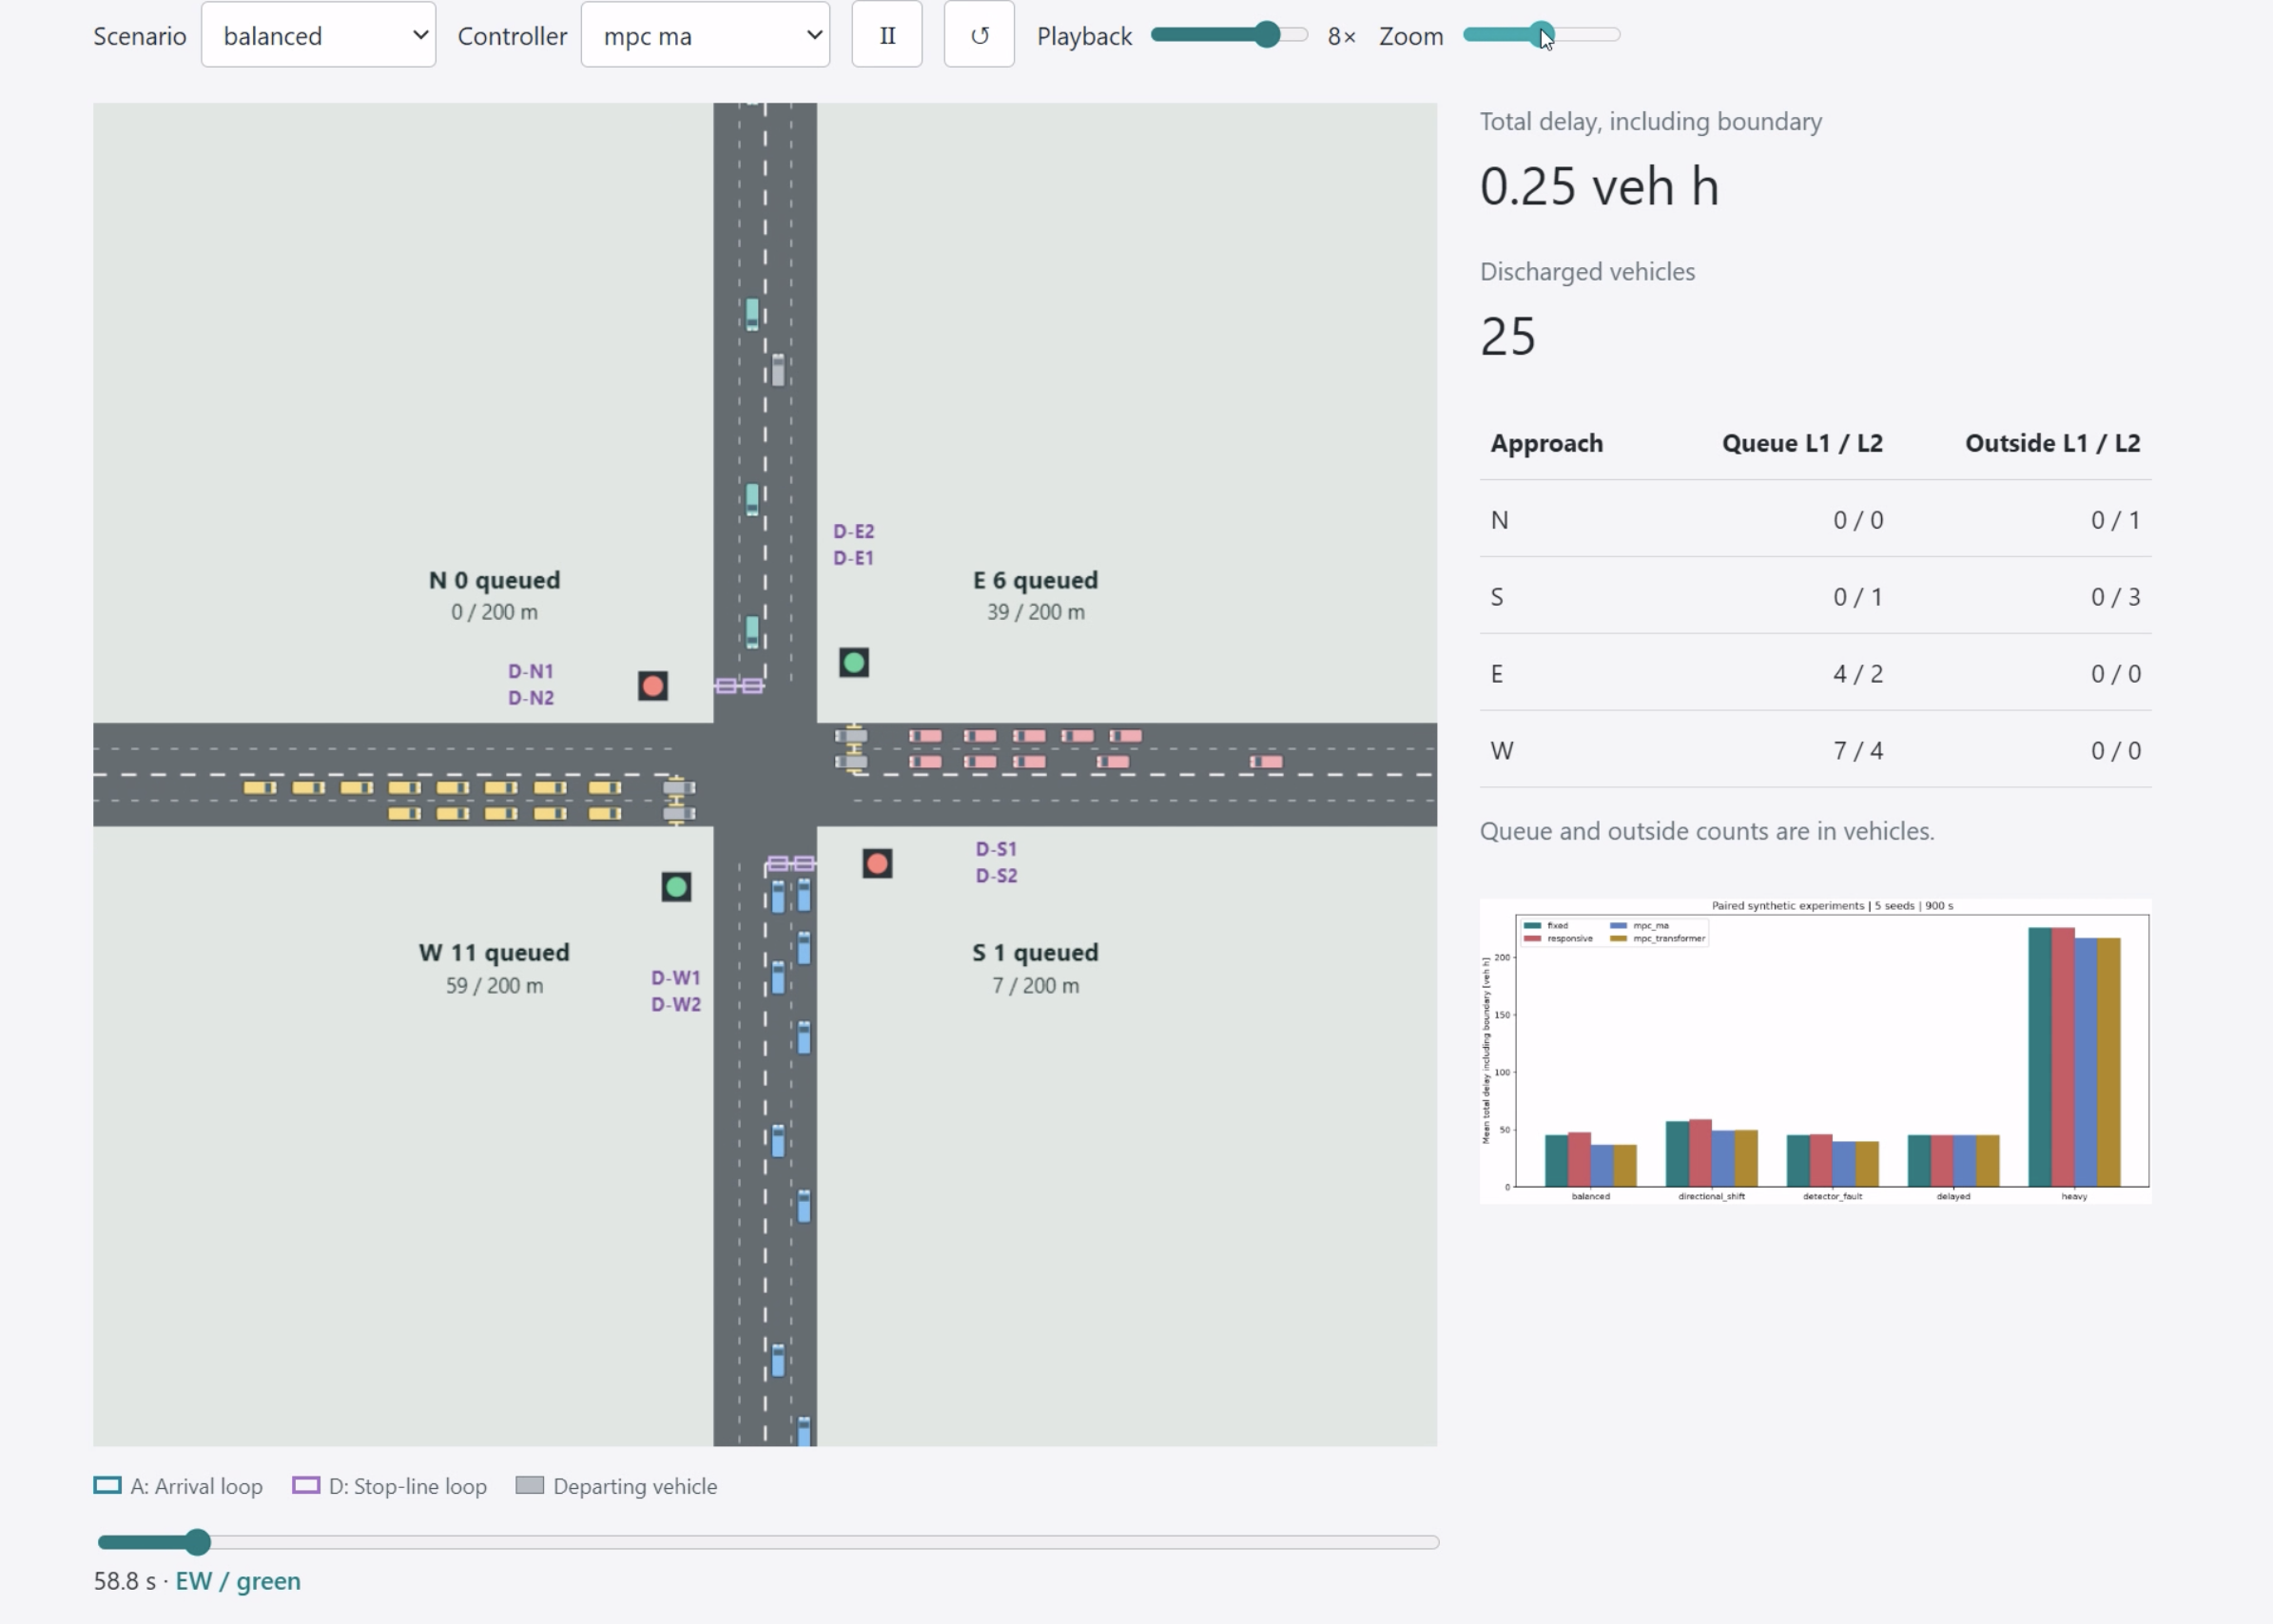
\includegraphics[width=\linewidth]{Simulation_Example.png}
    \caption{Initial simulation environment and results.}
    \label{fig:Simulation_Example}
\end{figure}

\subsection{Feasibility and Next Steps}

\begin{table}[t]
\caption{Simulation scenarios}
\label{tab:exp}
\centering
\footnotesize
\setlength{\tabcolsep}{3pt}
\begin{tabular}{p{0.27\linewidth}p{0.67\linewidth}}
\toprule
Scenario & Implementation \\
\midrule
Balanced demand & comparable average demand on all approaches;
direction split oscillates with a 300-s period \\
Directional shift & from 450~s, north/southbound demand rises and
east/westbound demand falls \\
Detector failure & reports missing from 360 to 585~s, or
delivered 30~s late \\
Heavy demand & balanced profile scaled by 2.1 \\
\bottomrule
\end{tabular}
\end{table}

As illustrated in Fig.~\ref{fig:Simulation_Example}, the intersection simulation, detectors, the three controllers, and result checks already run end to
end for the four scenarios in Table~\ref{tab:exp}. Each scenario
is simulated for 900~s, with identical demand realizations,
initial queues, and simulation horizons across controllers. The
main risks are the simplified queue model inside the optimizer and
the synthetic demand. Next, we will:
\begin{enumerate}
\item measure saturation flow from simulated queue discharge,
compare it with (\ref{eq:equil}), and use it in the optimizer;
\item justify the fixed-time plan with Webster's cycle;
\item implement the ablation without the forecast, and a
sensitivity study relating the Transformer's forecast error and
the observation delay to the resulting delay;
\item repeat all experiments with more random seeds and evaluate
total and approach-specific delay, throughput, maximum and
residual queue lengths, unmet demand, and service imbalance
between approaches, using summary statistics, 95\% confidence
intervals, and signal phase timelines with the corresponding
queue evolution, reporting every scenario including those without
improvement;

\end{enumerate}

%%%%%%%%%%%%%%%%%%%%%%%%%%%%%%%%%%%%%%%%%%%%%%%%%%%%%%%%%%%%
\begin{thebibliography}{99}
\footnotesize

\bibitem{treiber2013}
M. Treiber and A. Kesting, \textit{Traffic Flow Dynamics: Data,
Models and Simulation}. Berlin, Germany: Springer, 2013.

\bibitem{webster1958}
F. V. Webster, ``Traffic signal settings,'' Road Research
Laboratory, London, U.K., Road Research Tech. Paper No.~39, 1958.

\bibitem{newell1993}
G. F. Newell, ``A simplified theory of kinematic waves in highway
traffic, part I: General theory,'' \textit{Transp. Res. Part B},
vol.~27, no.~4, pp.~281--287, 1993.

\bibitem{lighthill1955}
M. J. Lighthill and G. B. Whitham, ``On kinematic waves II. A
theory of traffic flow on long crowded roads,'' \textit{Proc. R.
Soc. Lond. A}, vol.~229, no.~1178, pp.~317--345, 1955.

\bibitem{treiber2000}
M. Treiber, A. Hennecke, and D. Helbing, ``Congested traffic
states in empirical observations and microscopic simulations,''
\textit{Phys. Rev. E}, vol.~62, no.~2, pp.~1805--1824, 2000,
doi: 10.1103/PhysRevE.62.1805.

\bibitem{stm2015}
National Academies of Sciences, Engineering, and Medicine,
\textit{Signal Timing Manual, 2nd ed.} (NCHRP Rep.~812).
Washington, DC: The National Academies Press, 2015,
doi: 10.17226/22097.

\bibitem{kesting2010}
A. Kesting, M. Treiber, and D. Helbing, ``Enhanced intelligent
driver model to access the impact of driving strategies on traffic
capacity,'' \textit{Phil. Trans. R. Soc. A}, vol.~368, no.~1928,
pp.~4585--4605, 2010.

\bibitem{treiberweb}
M. Treiber, ``The Intelligent-Driver Model and its variants.''
traffic-simulation.de. Accessed: Oct.~18, 2026. [Online].
Available: https://traffic-simulation.de/info/info\_IDM.html

\bibitem{elkhouly2025}
M. ElKhouly, T. Alhadidi, and H. Rakha, ``Modeling traffic
vehicular counts at an urban intersection using complex seasonal
modeling techniques,'' \textit{KSCE J. Civ. Eng.}, vol.~29, no.~1,
art.~100040, 2025, doi: 10.1016/j.kscej.2024.100040.

\bibitem{vaswani2017}
A. Vaswani \textit{et al.}, ``Attention is all you need,'' in
\textit{Proc. Adv. Neural Inf. Process. Syst. (NeurIPS)}, vol.~30,
2017, pp.~5998--6008.

\bibitem{li2025}
Z. Li and K. Savla, ``Adaptive model predictive control for
traffic signal timing with unknown demand and parameters,''
arXiv:2503.10934, 2025.

\bibitem{atef2026}
S. Atef and A. Karam, ``An adaptive traffic signal control
framework integrating regime-aware LSTM forecasting and signal
optimization under socio-temporal demand shifts,''
\textit{Appl. Syst. Innov.}, vol.~9, no.~4, art.~81, 2026,
doi: 10.3390/asi9040081.

\bibitem{jia2025}
S. Jia, S. C. Wong, and W. Wong, ``Adaptive signal control at
partially connected intersections: A stochastic optimization model
for uncertain vehicle arrival rates,'' \textit{Transp. Res. Part B},
vol.~193, art.~103161, 2025, doi: 10.1016/j.trb.2025.103161.

\bibitem{varaiya2013}
P. Varaiya, ``Max pressure control of a network of signalized
intersections,'' \textit{Transp. Res. Part C}, vol.~36,
pp.~177--195, 2013, doi: 10.1016/j.trc.2013.08.014.

\end{thebibliography}

%%%%%%%%%%%%%%%%%%%%%%%%%%%%%%%%%%%%%%%%%%%%%%%%%%%%%%%%%%%%
\section*{APPENDIX}

\emph{Components.} Younggun Kim: Transformer forecasting model,
simulation development, evaluation, and report drafting. Manuel A.
Martinez Garcia: conceptualization, rolling-horizon optimizer,
evaluation, and report drafting and finalization. We jointly
designed the experiments, reviewed the full text, and are each
responsible for the whole submission.

\emph{AI-use disclosure.} Claude generated the initial
simulation code, documentation, and pilot synthetic experiments.
Claude was used to check our earlier draft against the
assignment and to restructure and edit this text from our
manuscript and code. We checked the equations, parameter values,
and citations against the code and sources, and we take
responsibility for the content.

\end{document}
